% =====================================================================
%  Praesentation Group 4 -- MA-Seminar "Meta-Analysis", UZH, HS 2026
%  Termin: Di 24.11.2026 | 20 Min. Vortrag + 10 Min. Diskussion
%
%  SKELETT: Struktur, Zeitbudget, Grafiken und Tabellen sind drin.
%  Alles in Orange ("TODO") muss noch ausformuliert werden.
%
%  Kompilieren (lokal, im Ordner 04_report/slides/):
%      latexmk -pdf slides.tex
%  Overleaf: slides.tex und Ordner sections/ hochladen; figures/, tables/
%  und references.bib entweder ins Root oder eine Ebene hoeher legen
%  (beide Varianten werden unten automatisch erkannt).
%
%  Zahlen NIE von Hand tippen: die Makros \ma... kommen aus
%  tables/macros_*.tex (erzeugt von 02_code/run_all.py).
%
%  Zeitplan (Soll; "bis" = Stand am Ende der Folie)
%  --------------------------------------------------------------------
%   #  Folie                                    Dauer    bis
%   1  Title                                     0:15    0:15
%   2  Roadmap                                   0:15    0:30
%      -- 1  Research question ------------------------------------
%   3  Motivation and research question         1:15    1:45
%   4  Correspondence tests: design and data    1:30    3:15
%   5  Estimating equation and effect size      1:30    4:45
%      -- 2  Original meta-analysis and replication -----------------
%   6  Zschirnt & Ruedin (2016)                 1:15    6:00
%   7  Replication                              1:30    7:30
%   8  Forest plot (original studies)           1:15    8:45
%      -- 3  Update --------------------------------------------------
%   9  New studies                              1:15   10:00  <- Halbzeit
%  10  Pooled estimate before / after           1:30   11:30
%      -- 4  Power and publication bias -----------------------------
%  11  Statistical power                        1:30   13:00
%  12  Funnel plot                              1:30   14:30
%  13  Bias-corrected estimates                 1:45   16:15
%      -- 5  Heterogeneity ------------------------------------------
%  14  WLS meta-regression                      1:45   18:00
%      -- 6  Conclusion ---------------------------------------------
%  15  Conclusion                               1:30   19:30
%  16  Thank you / discussion                   0:15   19:45  (+0:15 Puffer)
%  --------------------------------------------------------------------
%  Backup (Appendix, nur bei Fragen; Buttons auf den Hauptfolien,
%  "Back"-Button fuehrt zurueck):
%   A1  Replication, all estimators            <- Folie 7
%   A2  Forest plot incl. new studies          <- Folie 10
%   A3  Power robustness / weight of Kline     <- Folien 10 und 11
%   A4  Corrected estimates, all samples       <- Folie 13
% =====================================================================

\documentclass[aspectratio=169,11pt]{beamer}

\usepackage[T1]{fontenc}
\usepackage[utf8]{inputenc}
\usepackage{lmodern}
\usepackage{amsmath,amssymb}
\usepackage{booktabs,array}
\usepackage{graphicx}
\usepackage{adjustbox}
\usepackage{varwidth}
\usepackage[authoryear,round]{natbib}
\usepackage{appendixnumberbeamer}

% ---------- Schalter --------------------------------------------------
\newif\ifshowtiming
\showtimingtrue   % Zeitbudget in der Fusszeile (fuer Proben).
                  % Vor dem Mailen an den Prof: \showtimingfalse

% ---------- Pfade: lokal eine Ebene hoeher, auf Overleaf im Root ------
\IfFileExists{../tables/macros_replication.tex}{\def\repodir{../}}{\def\repodir{}}
\graphicspath{{../figures/}{figures/}}

% ---------- Zahlen aus der Analyse (\ma...) ---------------------------
\input{\repodir tables/macros_replication.tex}
\input{\repodir tables/macros_power_bias.tex}
\IfFileExists{\repodir tables/macros_update.tex}{\input{\repodir tables/macros_update.tex}}{}

% ---------- Layout ----------------------------------------------------
\usetheme{default}
\definecolor{uzhblue}{RGB}{0,40,165}
\definecolor{uzhgrey}{RGB}{110,110,110}
\definecolor{todocolor}{RGB}{214,90,0}
\setbeamercolor{structure}{fg=uzhblue}
\setbeamercolor{frametitle}{fg=uzhblue}
\setbeamercolor{title}{fg=uzhblue}
\setbeamercolor{footline}{fg=uzhgrey}
\setbeamercolor{keymsg}{bg=uzhblue!8,fg=black}
\setbeamerfont{frametitle}{series=\bfseries,size=\large}
\setbeamerfont{footline}{size=\scriptsize}
\setbeamertemplate{navigation symbols}{}
\setbeamertemplate{itemize items}[circle]
\setbeamertemplate{caption}{\raggedright\small\insertcaption\par}
\setbeamertemplate{bibliography item}{}
\setbeamertemplate{frametitle continuation}[from second]
\setbeamertemplate{footline}{%
  \leavevmode\hbox to \paperwidth{%
    \usebeamerfont{footline}\usebeamercolor[fg]{footline}%
    \hspace*{1.2em}\insertshortauthor\hfill
    \ifshowtiming\textcolor{todocolor}{\curtiming}\hfill\fi
    \insertframenumber\,/\,\inserttotalframenumber\hspace*{1.2em}}%
  \vspace*{1.2ex}}

% ---------- Hilfsbefehle ----------------------------------------------
% Zeitbudget einer Folie: \timing{Dauer}{Stand am Ende}
\gdef\curtiming{}
\newcommand{\timing}[2]{\gdef\curtiming{#1 min \textbar{} bis #2}}
% Platzhalter, der beim Kompilieren auffaellt
\newcommand{\todo}[1]{\textcolor{todocolor}{\textbf{TODO:} #1}}
% Kernaussage einer Folie (ein Satz), unten auf der Folie
\newcommand{\keymsg}[1]{\par\vfill
  \begin{beamercolorbox}[sep=0.5em,wd=\linewidth]{keymsg}#1\end{beamercolorbox}}
% Buttons: Hauptfolie -> Backup und Backup -> Hauptfolie
\newcommand{\gotobackup}[2]{\hyperlink{#1}{\beamergotobutton{#2}}}
\newcommand{\backto}[2]{\hyperlink{#1}{\beamerreturnbutton{#2}}}
\newcommand{\buttons}[1]{\par\vspace{0.3em}\hfill#1}
% Tabellen aus tables/ auf Folienformat skalieren:
%   \slidetable{datei}{max. Hoehe}       mit Titel und Anmerkungen
%   \slidetablebare{datei}{max. Hoehe}   ohne Titel und Anmerkungen
\newcommand{\slidetableaux}[3]{\begingroup#1%
  \begin{adjustbox}{max width=\linewidth,max totalheight=#3,center}%
    \begin{varwidth}{17cm}\input{\repodir tables/#2}\end{varwidth}%
  \end{adjustbox}\endgroup}
\newcommand{\slidetable}[2]{\slidetableaux{}{#1}{#2}}
\newcommand{\slidetablebare}[2]{\slidetableaux{%
  \renewcommand{\parbox}[2]{}\renewcommand{\caption}[1]{}}{#1}{#2}}

% ---------- Titel -----------------------------------------------------
\title{Ethnic Discrimination in Hiring}
\subtitle{A Replication and Update of Zschirnt and Ruedin (2016)}
\author[de Silva \& Allenspach]{Kevin de Silva \and Vanessa Allenspach}
\institute{Group 4 -- MA Seminar ``Meta-Analysis'', Prof.\ Rainer Winkelmann\\
  University of Zurich, Fall 2026}
\date{24 November 2026}

\begin{document}

\begin{frame}[plain]
  \titlepage
\end{frame}

\begin{frame}{Roadmap}
  \timing{0:15}{0:30}
  \tableofcontents
\end{frame}

% =====================================================================
% 1  Research question                 Folien 3-5 | 4:15 min | bis 4:45
% Inhalt: Bericht Kap. 1-2 (main.tex); Vorgaben aus instruction.pdf:
% X und Y klar benennen, typische Methode, Schaetzgleichung, Datensatz.
% =====================================================================
\section{Research question}

% ---------------------------------------------------------------------
\begin{frame}{Motivation and research question}
  \timing{1:15}{1:45}
  \begin{itemize}
    \item \todo{Hook: why ethnic discrimination in hiring matters (one sentence)}
    \item \textbf{Treatment $X$:} minority signal (e.g.\ the name) on an
      otherwise equivalent job application
    \item \textbf{Outcome $Y$:} call-back, i.e.\ an invitation to a job interview
    \item \textbf{Research question:} \todo{How large is ethnic discrimination
      at the hiring stage, and how reliable is the evidence?}
  \end{itemize}
  \keymsg{\todo{Key message of this slide in one sentence}}
\end{frame}

% ---------------------------------------------------------------------
\begin{frame}{Correspondence tests: design and a typical dataset}
  \timing{1:30}{3:15}
  \begin{columns}[T]
    \begin{column}{0.48\textwidth}
      \textbf{Design}
      \begin{itemize}
        \item \todo{Fictitious written applications to real job ads}
        \item \todo{Matched CVs; minority signal assigned at random
          $\Rightarrow$ causal effect}
        \item \todo{Limitation: only the first stage of hiring}
      \end{itemize}
    \end{column}
    \begin{column}{0.48\textwidth}
      \textbf{Typical dataset: \citet{bertrand2004}}
      \begin{itemize}
        \item \todo{Setting and sample size (cities, ads, CVs)}
        \item \todo{One row per application: call-back (0/1), ethnic
          signal, CV characteristics}
        \item \todo{Main result in one line}
      \end{itemize}
    \end{column}
  \end{columns}
  \keymsg{\todo{Key message of this slide in one sentence}}
\end{frame}

% ---------------------------------------------------------------------
\begin{frame}{Typical estimating equation and effect size}
  \timing{1:30}{4:45}
  \textbf{Primary studies} (linear probability model)
  \[
    \text{Callback}_{ij} = \alpha + \beta\,\text{Minority}_i
      + \gamma' X_{ij} + \varepsilon_{ij}
  \]
  \todo{What $\beta$ identifies and why (random assignment)}

  \medskip
  \textbf{Meta-analysis} (one estimate per study, from call-back counts)
  \[
    y_i = \ln OR_i = \ln \frac{a_i/b_i}{c_i/d_i},
    \qquad
    SE_i = \sqrt{\frac{1}{a_i} + \frac{1}{b_i} + \frac{1}{c_i} + \frac{1}{d_i}}
  \]
  \todo{Define $a_i, b_i$ (minority: call-back yes / no) and $c_i, d_i$ (majority)}\\
  \todo{Sign: $OR < 1$, i.e.\ $y_i < 0$, means discrimination}
  \keymsg{\todo{Key message of this slide in one sentence}}
\end{frame}

% =====================================================================
% 2  Original meta-analysis and replication
%                                      Folien 6-8 | 4:00 min | bis 8:45
% Inhalt: Bericht Kap. 3-4. Backup A1 (alle Schaetzer) ist verlinkt.
% =====================================================================
\section{Original meta-analysis and replication}

% ---------------------------------------------------------------------
\begin{frame}{The original meta-analysis: \citet{zschirnt2016}}
  \timing{1:15}{6:00}
  \begin{itemize}
    \item \todo{Selection: correspondence tests in OECD countries,
      testing years 1990--2015, written applications only}
    \item \todo{Sample: 43 studies; \maK{} studies (\maKsub{} subgroups)
      report call-back counts and enter the pooled odds ratio}
    \item \todo{Method: random effects (REML), one estimate per study}
    \item \todo{Main result: OR \maORre{} \maCIre}
  \end{itemize}
  \keymsg{\todo{Key message of this slide in one sentence}}
\end{frame}

% ---------------------------------------------------------------------
\begin{frame}[label=replication]{Replication of the pooled effect ($k = \maK$)}
  \timing{1:30}{7:30}
  \centering
  \begin{tabular}{lccc}
    \toprule
    Model & OR [95\% CI] & $\hat\tau^2$ & $I^2$ (\%) \\
    \midrule
    Fixed effect (FE)     & \maORfe{} \maCIfe     & -- & -- \\
    UWLS                  & \maORuwls{} \maCIuwls & -- & -- \\
    Random effects (REML) & \maORre{} \maCIre     & \maTauSqRe & \maIsqRe \\
    \midrule
    \citet{zschirnt2016}, RE (REML) & 0.60 [0.52; 0.69] & 0.141 & 92.7 \\
    \bottomrule
  \end{tabular}

  \raggedright
  \begin{itemize}
    \item \todo{Replication is exact}
    \item \todo{Same point estimate for FE and UWLS, but UWLS SE is
      \maSEratioUWLS{} times larger $\Rightarrow$ heterogeneity}
  \end{itemize}
  \keymsg{\todo{Key message of this slide in one sentence}}
  \buttons{\gotobackup{app-replication}{All estimators}}
\end{frame}

% ---------------------------------------------------------------------
\begin{frame}{Forest plot: original studies}
  \timing{1:15}{8:45}
  \begin{columns}[T]
    \begin{column}{0.56\textwidth}
      \centering
      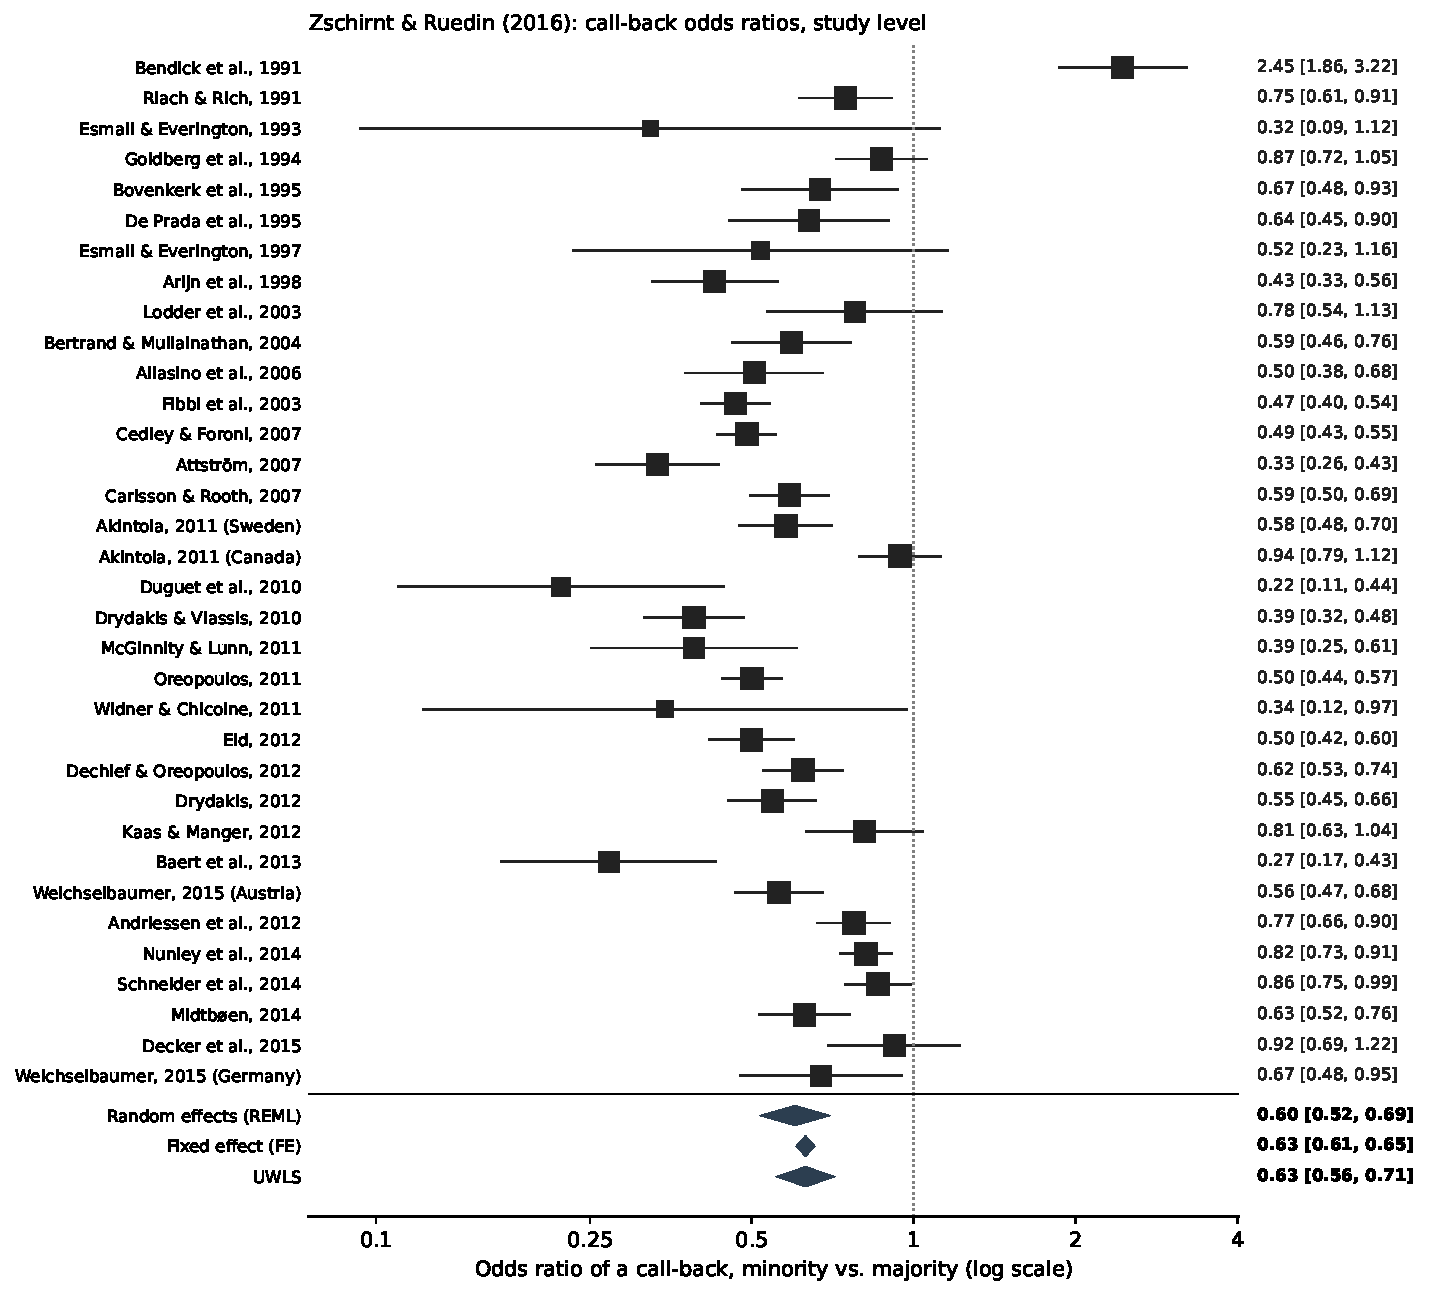
\includegraphics[height=0.82\textheight]{forest_original}
    \end{column}
    \begin{column}{0.42\textwidth}
      \begin{itemize}
        \item \todo{What the plot shows: direction, spread, outliers}
        \item \todo{Heterogeneity: $I^2 = \maIsqRe\,\%$; prediction
          interval \maPIre{} includes 1}
        \item \todo{Outlier Bendick et al.\ (1991): kept in the main
          model, as in the original}
      \end{itemize}
      \medskip
      \todo{Key message}
    \end{column}
  \end{columns}
\end{frame}

% =====================================================================
% 3  Update with new studies           Folien 9-10 | 2:45 min | bis 11:30
% Inhalt: Bericht Kap. 5. Halbzeit nach Folie 9 (ca. 10:00).
% Backup A2 (Forest Plot mit neuen Studien) und A3 (Gewicht Kline) verlinkt.
% =====================================================================
\section{Update with new studies}

% ---------------------------------------------------------------------
\begin{frame}{Update: \maKnew{} more recent correspondence tests}
  \timing{1:15}{10:00}
  \todo{How the new studies were selected (same criteria as the original)}

  \medskip
  \slidetable{update_new_studies}{0.5\textheight}
  \keymsg{\todo{Do the new estimates lie in the original CI? (\maNnewInCI{}
    of \maKnew{} inside the CI)}}
\end{frame}
% ------------------------- Halbzeit (ca. 10:00) -----------------------

% ---------------------------------------------------------------------
\begin{frame}[label=update]{Does the update change the pooled estimate?}
  \timing{1:30}{11:30}
  \slidetablebare{update_pooled}{0.3\textheight}
  \begin{itemize}
    \item \todo{RE barely moves: \maORre{} $\to$ \maORcomb}
    \item \todo{FE and UWLS move strongly: \maORuwls{} $\to$ \maORuwlsComb.
      Why? \citet{kline2022} gets \maWshareKline\,\% of the UWLS weight,
      but only \maWshareKlineRE\,\% of the RE weight}
  \end{itemize}
  \keymsg{\todo{Key message of this slide in one sentence}}
  \buttons{\gotobackup{app-forest}{Forest plot incl.\ new studies}\quad
    \gotobackup{app-power}{Weight of Kline et al.}}
\end{frame}

% =====================================================================
% 4  Power and publication bias        Folien 11-13 | 4:45 min | bis 16:15
% Inhalt: Bericht Kap. 6-7. Pflicht laut instruction.pdf: Funnel Plot und
% eine Aussage zur visuellen Evidenz fuer Publication bias.
% Backup A3 (Power-Robustheit) und A4 (alle Stichproben) verlinkt.
% Von Hand getippte Zahlen (kein Makro) sind unten markiert.
% =====================================================================
\section{Power and publication bias}

% ---------------------------------------------------------------------
\begin{frame}[label=power]{Statistical power}
  \timing{1:30}{13:00}
  \begin{columns}[T]
    \begin{column}{0.55\textwidth}
      \centering
      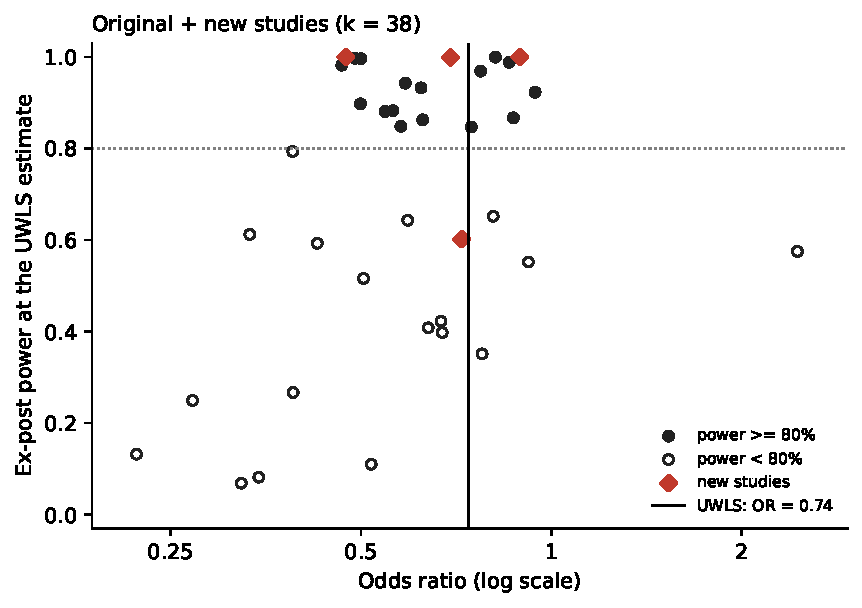
\includegraphics[width=\linewidth]{power_combined}
    \end{column}
    \begin{column}{0.43\textwidth}
      \[ q_i = \Phi\!\left( \frac{|\hat\mu_{UWLS}|}{SE_i} - 1.96 \right) \]
      \begin{itemize}
        \item \textbf{Median power:} \maMedPower{} (original),
          \maMedPowerComb{} (with new studies)
        \item \textbf{Adequately powered} ($q_i \geq 0.8$): \maNadequate{}
          of \maK{} / \maNadequateComb{} of \maKcomb
        \item Leading economics journals: median power only 7\,\%
          \citep{askarov2024}% 7 % von Hand (Bericht Kap. 6)
      \end{itemize}
    \end{column}
  \end{columns}
  \keymsg{Correspondence tests are well powered; the drop after the update
    reflects a smaller benchmark effect, not weaker studies.}
  \buttons{\gotobackup{app-power}{Robustness}}
\end{frame}
% Sprechnotizen (Folie 11):
% - Grafik: jeder Punkt = eine Studie; x = OR, y = Power; gestrichelt = 80 %.
% - Formel: wahrer Effekt = UWLS-Schaetzer. Adequately powered heisst
%   SE_i <= |mu| / 2.8 (1.96 + 0.84 = 2.8).
% - Warum sinkt die Power nach dem Update? Kline zieht UWLS gegen 1; ein
%   kleinerer angenommener Effekt senkt die Power ALLER Studien. Ohne Kline:
%   Median 0.99 (Backup A3).
% - Einschraenkung: eher Obergrenze (nur publizierte Studien; der
%   Benchmark-Effekt kann selbst durch Publication bias aufgeblaeht sein).

% ---------------------------------------------------------------------
\begin{frame}{Publication bias: visual evidence}
  \timing{1:30}{14:30}
  \begin{columns}[T]
    \begin{column}{0.58\textwidth}
      \centering
      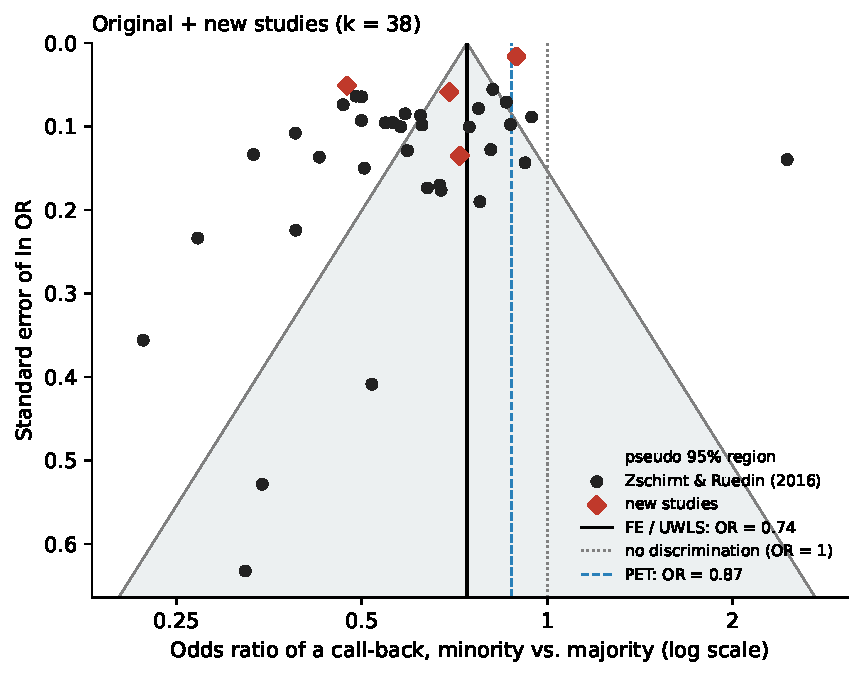
\includegraphics[width=0.92\linewidth]{funnel_combined}
    \end{column}
    \begin{column}{0.40\textwidth}
      \begin{itemize}
        \item \textbf{Asymmetric:} 15 of 19 less precise studies lie left of
          the UWLS estimate, i.e.\ report stronger discrimination% 15 of 19 von Hand (Bericht Kap. 7)
        \item \textbf{New studies} (red): three are among the four most
          precise studies, yet range from \maORnewMin{} to \maORnewMax
        \item \textbf{Caveat:} with $\ln OR$, effect and SE are
          mechanically correlated
      \end{itemize}
    \end{column}
  \end{columns}
  \keymsg{Asymmetric funnel: consistent with publication bias, but also with
    heterogeneity.}
\end{frame}
% Sprechnotizen (Folie 12):
% - Lesen: oben praezise, unten unpraezise Studien. Ohne Bias symmetrisch
%   um die durchgezogene Linie (FE/UWLS 0.74). Blau gestrichelt = PET (0.87),
%   gepunktet = OR 1 (keine Diskriminierung).
% - Viele praezise Studien liegen ausserhalb des grauen Pseudo-95%-Bereichs
%   -> grosse Heterogenitaet.
% - Neue Studien: Kline (Rang 1), Adamovic (2) und Koopmans (4) sind sehr
%   praezise; Zschirnt & Fibbi liegt in der unpraeziseren Haelfte (Rang 24).
% - Caveat: der SE haengt von den Callback-Zahlen ab, diese von der
%   Callback-Rate -> Asymmetrie ist kein Beweis fuer Bias.

% ---------------------------------------------------------------------
\begin{frame}[label=bias]{Correcting for publication bias}
  \timing{1:45}{16:15}
  \vspace{-0.5em}
  \[
    y_i = \beta_0 + \beta_1 SE_i + \varepsilon_i, \quad w_i = 1/SE_i^2
    \qquad \text{FAT: } H_0\!: \beta_1 = 0, \quad \text{PET: } \hat\beta_0
  \]
  \centering\small
  \begin{tabular}{lcc}
    \toprule
    & Original ($k = \maK$) & Original + new ($k = \maKcomb$) \\
    \midrule
    RE (REML), OR      & \maORre{} \maCIre       & \maORcomb{} \maCIcomb \\
    WAAP, OR           & \maORwaap{} \maCIwaap   & \maORwaapComb{} \maCIwaapComb \\
    PET, OR            & \maORpet{} \maCIpet     & \maORpetComb{} \maCIpetComb \\
    FAT: $\hat\beta_1$ (SE) & \maFAT{} (\maFATse) & \maFATComb{} (\maFATseComb) \\
    ESS (observed $-$ expected) & \maESS        & \maESSComb \\
    \bottomrule
  \end{tabular}

  \raggedright\normalsize
  \begin{itemize}
    \item \textbf{Original:} FAT insignificant, ESS $\approx 0$
      $\Rightarrow$ little sign of bias
    \item \textbf{With new studies:} significant FAT, excess significance,
      PET moves to \maORpetComb{} -- driven by \citet{kline2022}
  \end{itemize}
  \keymsg{Evidence of bias appears only once the very precise US study is
    included; all corrected estimates stay below 1.}
  \buttons{\gotobackup{app-bias}{All samples}}
\end{frame}
% Sprechnotizen (Folie 13) -- schwierigste Folie, Zeit nehmen:
% - FAT (beta_1): Bei Diskriminierung ist ln OR < 0. Eine unpraezise Studie
%   braucht einen STAERKER negativen Effekt, um signifikant zu sein. Wird
%   nur Signifikantes publiziert -> beta_1 < 0. Kombiniert: -3.16 (SE 0.86).
% - PET (beta_0): Effekt einer hypothetischen Studie mit SE -> 0 = korrigierter Effekt.
% - WAAP: UWLS nur ueber Studien mit Power >= 80 %; aendert kaum etwas
%   (0.76 vs. 0.74), weil UWLS die schwachen Studien ohnehin kaum gewichtet.
% - ESS: 31 von 38 signifikant (0.82), erwartet laut Power nur 0.68.
% - Muendlich (von Hand gerechnet, nicht auf der Folie): ohne Kline ist die
%   Steigung -0.40 (SE 1.21), nicht signifikant, PET-OR 0.64.

% =====================================================================
% 5  Heterogeneity                     Folie 14 | 1:45 min | bis 18:00
% Inhalt: Bericht Kap. 8. Pflicht laut instruction.pdf: WLS-Meta-
% Regression zu Publication bias und (falls moeglich) Heterogenitaet.
% =====================================================================
\section{Sources of heterogeneity}

% ---------------------------------------------------------------------
\begin{frame}{Sources of heterogeneity: WLS meta-regression}
  \timing{1:45}{18:00}
  \vspace{-0.6em}
  {\small\[
    y_i = \beta_0 + \beta_1 SE_i + \textstyle\sum_k \delta_k Z_{ik}
      + \varepsilon_i, \qquad w_i = 1/SE_i^2
  \]}
  \vspace{-1.2em}
  \slidetablebare{metareg_wls}{0.6\textheight}
  \keymsg{Europe: stronger discrimination. Controlling for region shrinks the
    FAT (M1 $\to$ M2) $\Rightarrow$ part of the asymmetry is heterogeneity.}
\end{frame}
% Sprechnotizen (Folie 14) -- Zahlen aus der Tabelle, nicht auf der Folie getippt:
% - Lesen: Koeffizienten auf der ln-OR-Skala, negativ = mehr Diskriminierung.
%   Referenzgruppe: ausserhalb Europas, gemischte Skills, Testjahr 2000.
% - Europe: -0.28 (SE 0.13) in M2 -> OR ca. 25 % tiefer; stabil in M2-M5.
% - FAT faellt von -3.16 (M1) auf -1.91 (M2): europaeische Studien sind im
%   Schnitt unpraeziser UND finden mehr Diskriminierung -> ein Teil der
%   Funnel-Asymmetrie ist Zusammensetzung der Stichprobe.
% - Nicht signifikant: German-speaking (+0.20), Skills (M3, nur k = 30),
%   Zeittrend (-0.01), Dummy neue Studien (0.04).
% - Caveat: nur 38 Studien, korrelierte Moderatoren, vieles bleibt unerklaert.

% =====================================================================
% 6  Conclusion                        Folien 15-16 | 1:45 min | bis 19:45
% Inhalt: Bericht Kap. 9 (Aufgabe 6: is there reliable evidence on the
% true effect size?). Restliche ca. 15 s = Puffer.
% =====================================================================
\section{Conclusion}

% ---------------------------------------------------------------------
\begin{frame}{Conclusion: is the evidence reliable?}
  \timing{1:30}{19:30}
  \begin{itemize}
    \item \textbf{Existence:} robust -- all pooled and corrected estimates
      are below 1, even the most conservative (PET, combined:
      \maORpetComb{} \maCIpetComb)
    \item \textbf{Magnitude:} uncertain -- estimates range from \maORsub{}
      to \maORpetComb; $I^2 = \maIsqRe\,\%$, prediction interval \maPIre{}
      includes 1
    \item \textbf{Publication bias:} little sign in the original sample; in
      the combined sample driven by one study and partly by region
    \item \textbf{Power:} high by economics standards (median \maMedPower),
      but likely an upper bound
    \item \textbf{Limitations:} reconstructed counts for three new studies;
      SEs ignore clustering by employer; only the first stage of hiring
  \end{itemize}
  \keymsg{Ethnic discrimination in hiring is robust, but its size varies
    strongly across countries and groups -- a single true effect is hard to
    justify.}
\end{frame}
% Sprechnotizen (Folie 15):
% - Pro Zeile ein Satz, sonst reichen 1:30 nicht.
% - Magnitude: Spannweite von 0.55 (RE, Subgruppen) bis 0.87 (PET, kombiniert).
%   Das Prediction Interval schliesst 1 ein -> in manchen Arbeitsmaerkten
%   kaum oder keine Diskriminierung.
% - Limitations: Bei Zeitdruck nur zwei nennen.

% ---------------------------------------------------------------------
\begin{frame}[c]
  \timing{0:15}{19:45}
  \centering
  {\usebeamercolor[fg]{structure}\Large\bfseries Thank you!}\\[1em]
  Questions and discussion\\[2.5em]
  {\small Kevin de Silva \quad\textbar\quad Vanessa Allenspach}
\end{frame}
% Vor dem Mailen an den Prof: in slides.tex \showtimingfalse setzen.


% =====================================================================
\appendix
\gdef\curtiming{}   % im Backup keine Zeitangaben
% =====================================================================
% Appendix / Backup -- nur bei Fragen in der Diskussion zeigen.
% Seitenzahlen zaehlen nicht zur Gesamtzahl (appendixnumberbeamer).
%
% Neue Backup-Folie anlegen:
%   1. hier: \begin{frame}[label=app-xyz]{Backup: ...} ... \end{frame}
%      mit \buttons{\backto{<label der Hauptfolie>}{Back}}
%   2. auf der Hauptfolie: [label=...] setzen und
%      \buttons{\gotobackup{app-xyz}{Text}}
% =====================================================================

% ---------------------------------------------------------------------
\begin{frame}[allowframebreaks]{References}
  \scriptsize
  \nocite{zschirnt2016,koopmans2019,kline2022,zschirnt2019,adamovic2023}
  \bibliographystyle{apalike}
  \bibliography{\repodir references}
\end{frame}

% ---------------------------------------------------------------------
% A1 <- Folie 7 (Replication)
\begin{frame}[label=app-replication]{Backup: replication with all estimators}
  \slidetable{replication}{0.75\textheight}
  \buttons{\backto{replication}{Back to replication}}
\end{frame}

% ---------------------------------------------------------------------
% A2 <- Folie 10 (Update)
\begin{frame}[label=app-forest]{Backup: forest plot including the new studies}
  \centering
  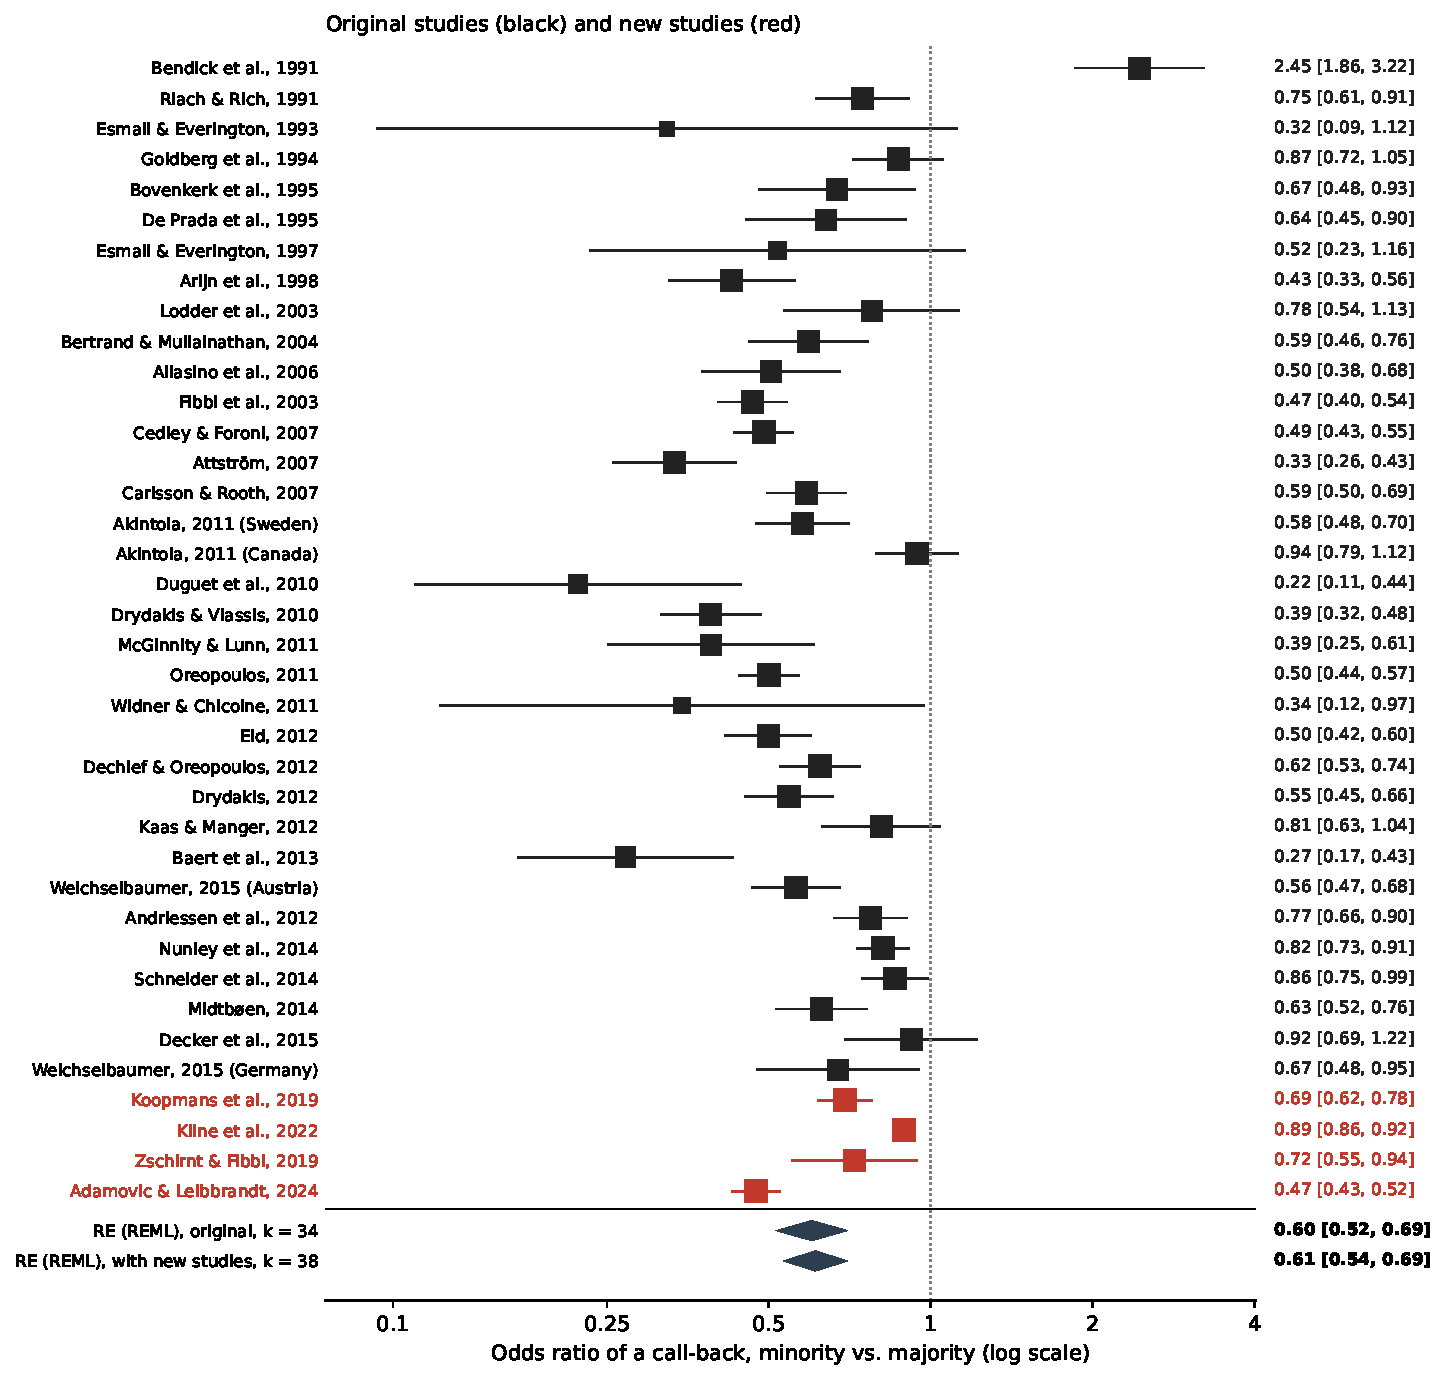
\includegraphics[height=0.8\textheight]{forest_combined}
  \buttons{\backto{update}{Back to update}}
\end{frame}

% ---------------------------------------------------------------------
% A3 <- Folien 10 (Update) und 11 (Power)
\begin{frame}[label=app-power]{Backup: power robustness and the weight of \citet{kline2022}}
  \slidetable{power_robustness}{0.7\textheight}
  \buttons{\backto{update}{Back to update}\quad\backto{power}{Back to power}}
\end{frame}

% ---------------------------------------------------------------------
% A4 <- Folie 13 (Publication bias)
\begin{frame}[label=app-bias]{Backup: pooled and corrected estimates for all samples}
  \slidetable{pubbias_estimates}{0.72\textheight}
  \buttons{\backto{bias}{Back to publication bias}}
\end{frame}


\end{document}
